\documentclass[border=12pt]{standalone}
\usepackage{tikz}
\usetikzlibrary{shapes.geometric, arrows.meta, positioning, calc, fit, backgrounds}
\usepackage{fontspec}
\usepackage{amsmath,amssymb}
\setmainfont{DejaVu Sans}

\begin{document}
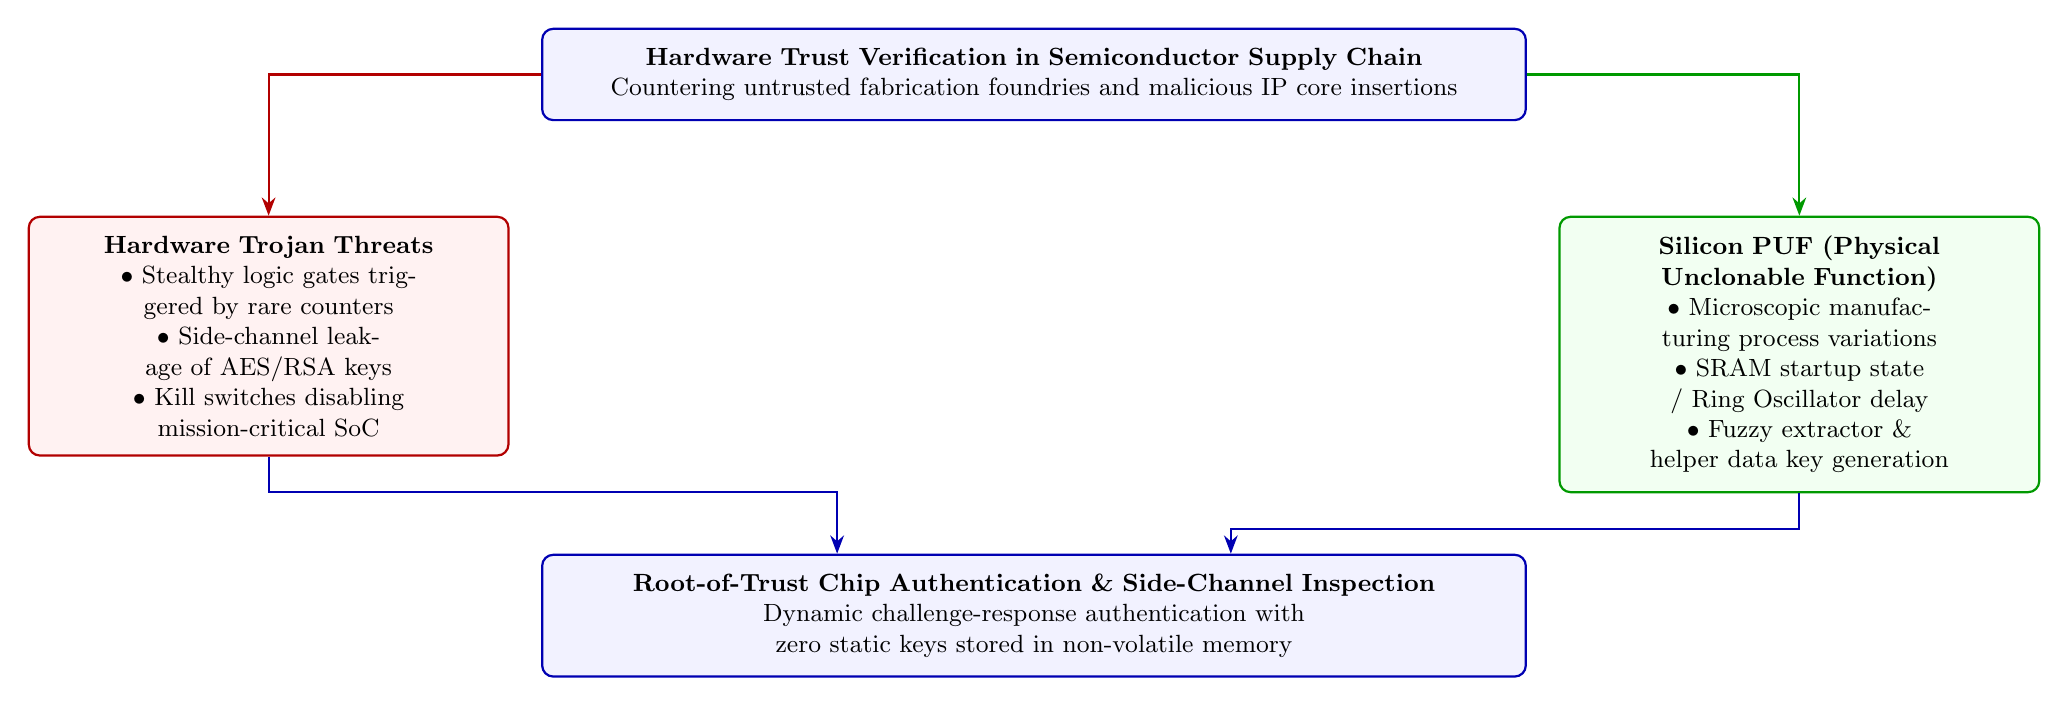
\begin{tikzpicture}[
    font=\small,
    >=Stealth,
    node distance=1.2cm,
    block/.style={rectangle, draw=blue!70!black, fill=blue!5, rounded corners=4pt, thick, align=center, inner sep=7pt},
    alertblock/.style={rectangle, draw=red!70!black, fill=red!5, rounded corners=4pt, thick, align=center, inner sep=7pt},
    greenblock/.style={rectangle, draw=green!60!black, fill=green!5, rounded corners=4pt, thick, align=center, inner sep=7pt},
    amberblock/.style={rectangle, draw=orange!80!black, fill=orange!5, rounded corners=4pt, thick, align=center, inner sep=7pt}
]

\node[block, text width=12cm] (top) {\textbf{Hardware Trust Verification in Semiconductor Supply Chain}\\Countering untrusted fabrication foundries and malicious IP core insertions};

\node[alertblock, below left=1.2cm and 0.4cm of top, text width=5.6cm] (trojan) {\textbf{Hardware Trojan Threats}\\$\bullet$ Stealthy logic gates triggered by rare counters\\$\bullet$ Side-channel leakage of AES/RSA keys\\$\bullet$ Kill switches disabling mission-critical SoC};

\node[greenblock, below right=1.2cm and 0.4cm of top, text width=5.6cm] (puf) {\textbf{Silicon PUF (Physical Unclonable Function)}\\$\bullet$ Microscopic manufacturing process variations\\$\bullet$ SRAM startup state / Ring Oscillator delay\\$\bullet$ Fuzzy extractor \& helper data key generation};

\node[block, below=1.0cm of $(trojan.south)!0.5!(puf.south)$, text width=12cm] (bottom) {\textbf{Root-of-Trust Chip Authentication \& Side-Channel Inspection}\\Dynamic challenge-response authentication with zero static keys stored in non-volatile memory};

\draw[->, thick, red!70!black] (top) -| (trojan);
\draw[->, thick, green!60!black] (top) -| (puf);
\draw[->, thick, blue!70!black] (trojan.south) -- ++(0,-0.45) -| ([xshift=-2.5cm]bottom.north);
\draw[->, thick, blue!70!black] (puf.south) -- ++(0,-0.45) -| ([xshift=2.5cm]bottom.north);

\end{tikzpicture}
\end{document}
